\documentclass[a4paper, 11pt]{article}
    \usepackage[utf8]{inputenc}
    \usepackage[english]{babel}
    \usepackage[breakable]{tcolorbox}
    \usepackage{indentfirst}
    \usepackage{graphicx}
    \usepackage{hyperref}
    \usepackage{color} 
    \usepackage{multirow}
    \usepackage{iftex}
    \ifPDFTeX
    	\usepackage[T1]{fontenc}
    	\usepackage{mathpazo}
    \else
    	\usepackage{fontspec}
    \fi
    \usepackage{caption}
    \DeclareCaptionFormat{nocaption}{}
    \captionsetup{format=nocaption,aboveskip=0pt,belowskip=0pt}

    \usepackage{float}
    \floatplacement{figure}{H} % forces figures to be placed at the correct location
    \usepackage{xcolor} % Allow colors to be defined
    \usepackage{enumerate} % Needed for markdown enumerations to work
    \usepackage{geometry} % Used to adjust the document margins
    \usepackage{amsmath} % Equations
    \usepackage{amssymb} % Equations
    \usepackage{textcomp} % defines textquotesingle


    \title{xklemr00\_knn\_project\_documentation}
    
    % Colors for the hyperref package
    \definecolor{urlcolor}{rgb}{0,.145,.698}
    \definecolor{linkcolor}{rgb}{.71,0.21,0.01}
    \definecolor{citecolor}{rgb}{.12,.54,.11}

    % Prevent overflowing lines due to hard-to-break entities
    \sloppy 
    % Setup hyperref package
    \hypersetup{
      breaklinks=true,  % so long urls are correctly broken across lines
      colorlinks=true,
      urlcolor=urlcolor,
      linkcolor=linkcolor,
      citecolor=citecolor,
      }
    % Slightly bigger margins than the latex defaults

    \geometry{verbose,tmargin=1in,bmargin=1in,lmargin=1in,rmargin=1in}
    
    
\begin{document}
    \begin{titlepage}
 \begin{center}
  {\Huge\textsc{Brno University of Technology\\[0.3em]
    \huge{Faculty of Information Technology}}}\\
  \vspace{\stretch{0.382}}
  {\Huge
  Generative image inpainting enhanced with edge focused WGAN-GP adversarial loss.}
  \vspace{\stretch{0.618}}
 \end{center}
 {\Large 
 \today 
 \hfill
%  TBD autori zde?
}
\end{titlepage}

\newpage
\section{Abstract}
\label{section:abstract}

\section{Introduction}
\label{section:introduction}

\section{The original work and article}
\label{section:origin}
    \begin{figure}
        \centering
        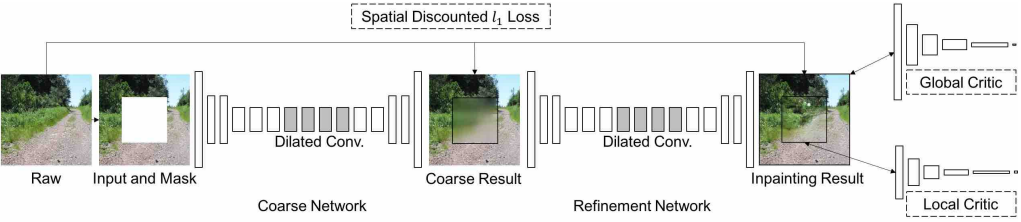
\includegraphics[width=0.95\linewidth]{documentation/img/original_arch.png}
    \end{figure}


\section{Edge focused discriminator}
\label{section:edgeDiscriminator}
    \begin{figure}
        \centering
        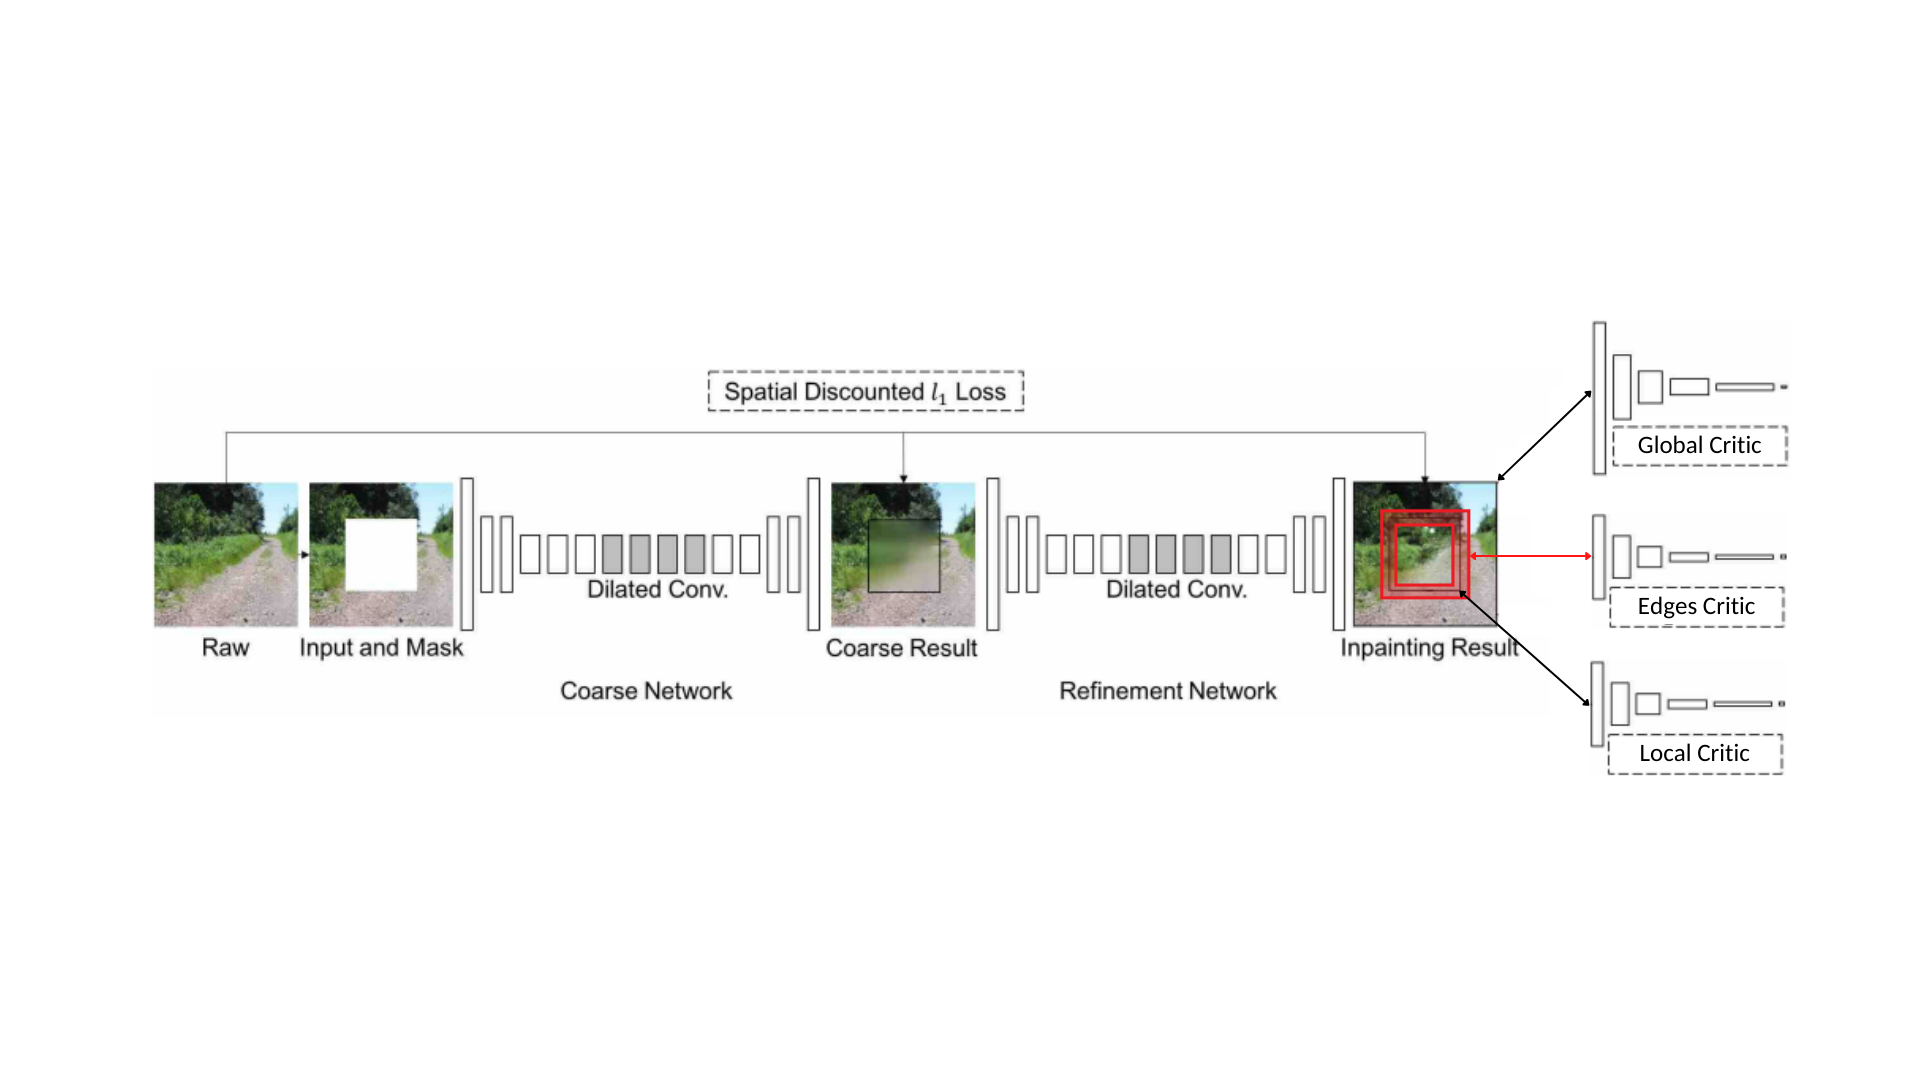
\includegraphics[width=0.95\linewidth]{documentation/img/new_arch.png}
    \end{figure}


\end{document}
